% Homework 4.tex 

\documentclass{article}
\usepackage{graphicx} % for figures
\usepackage{float}
\usepackage[export]{adjustbox}
\usepackage{fancyhdr}
\begin{document}

\title{Homework Work 5 - Physics 240}
\author{Tin Tran}

\maketitle

\section{The driven pendulum}

This is an excerise to calculate and plot the driven pendulum that has a time-varrying acceleration of the pivot. Below are some of the plots generated from the code with different values for $\theta$ and period $T$

\begin{figure}[H]
\centering{
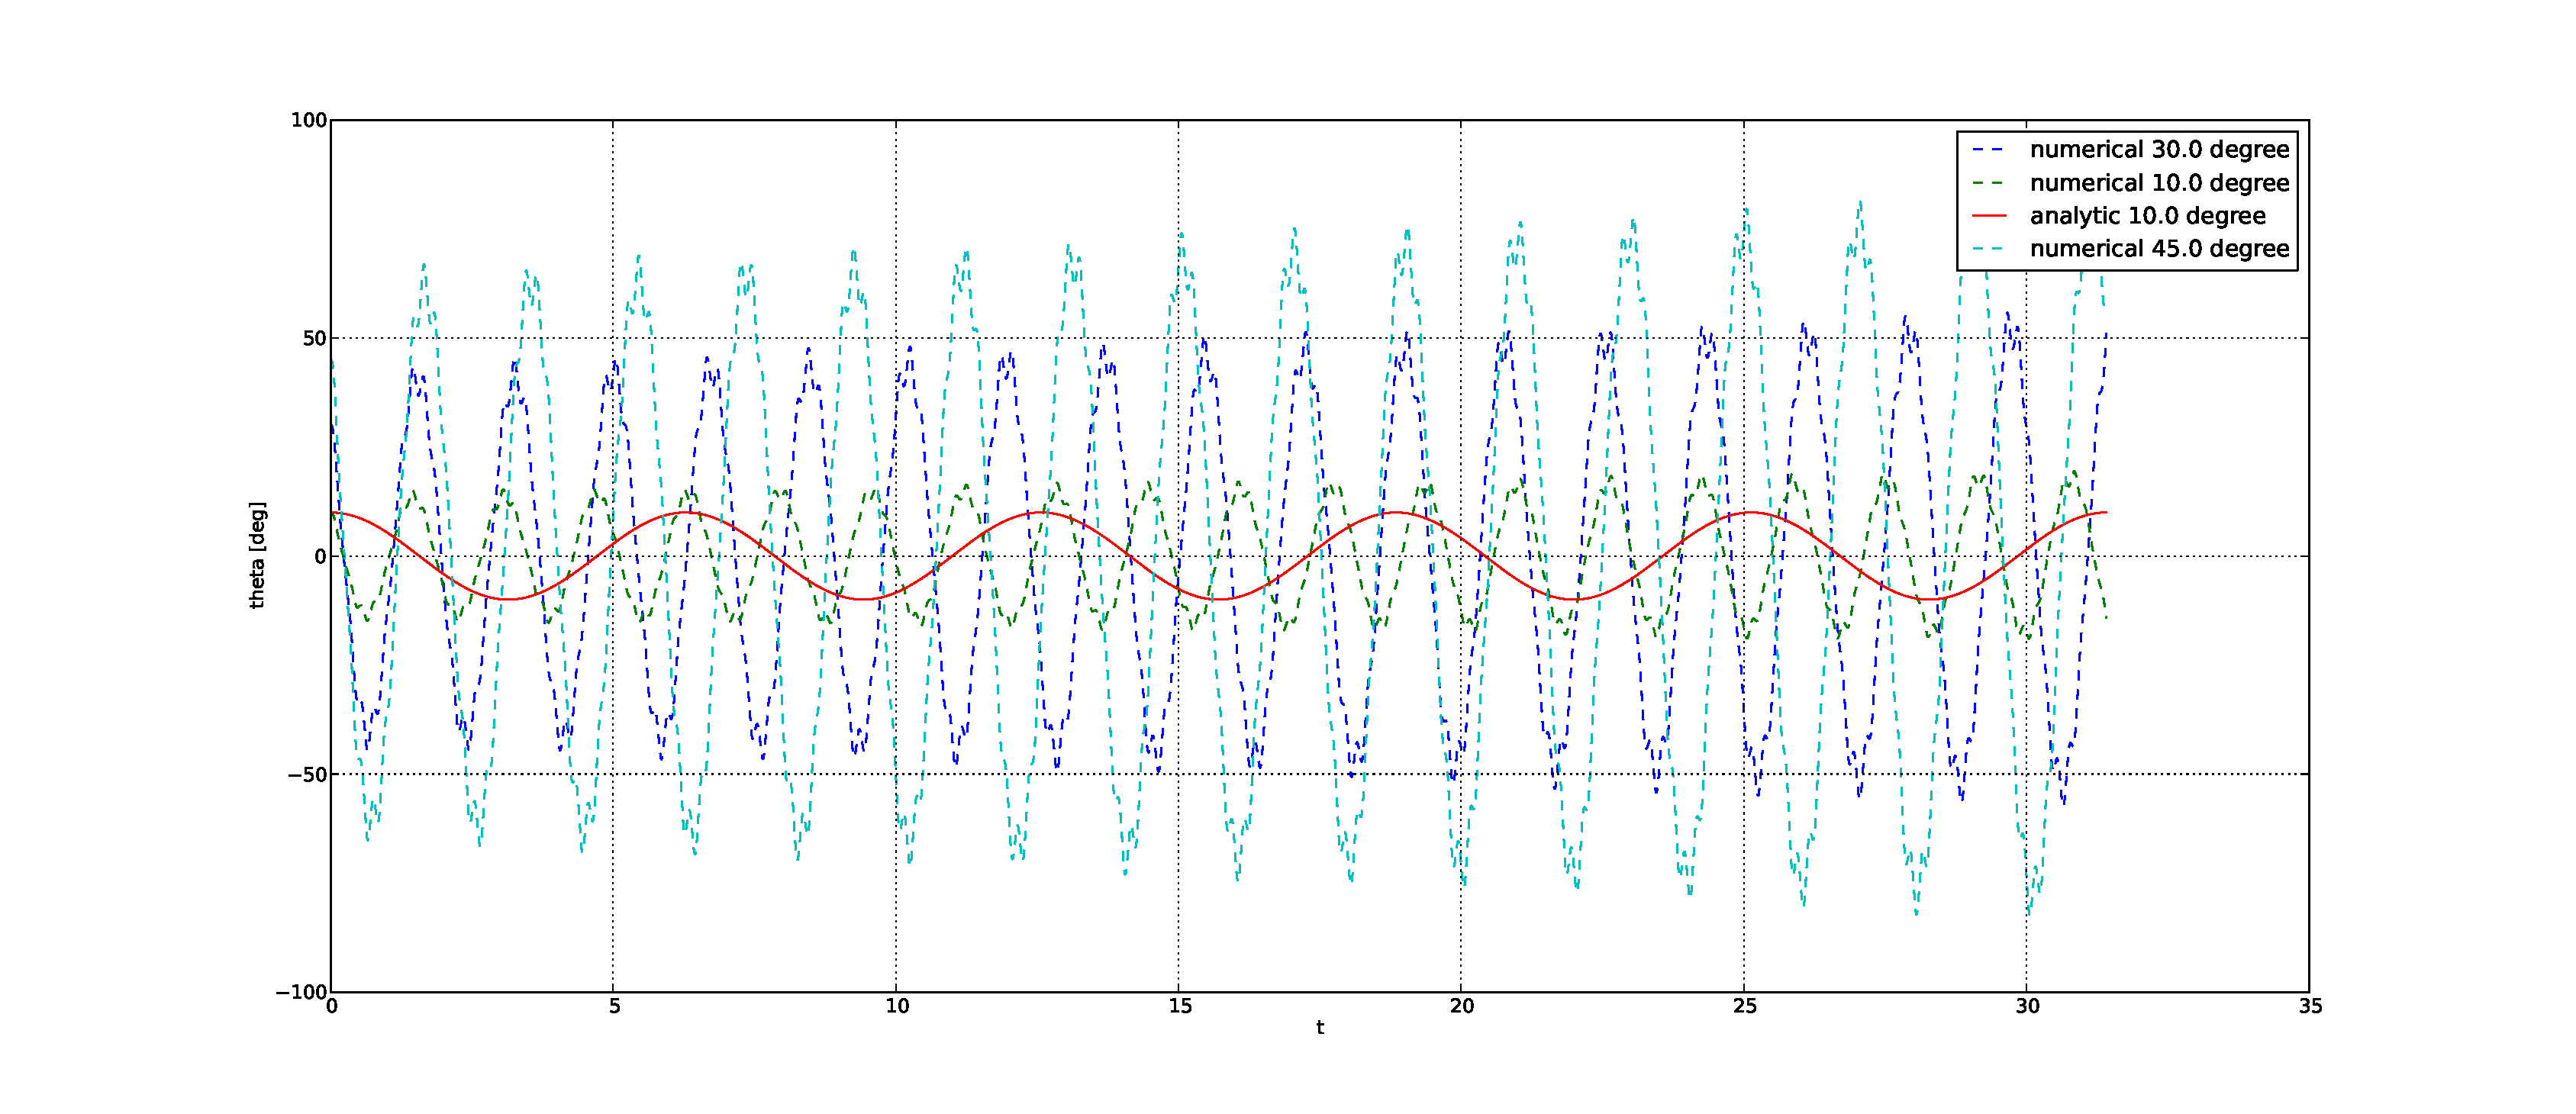
\includegraphics[max size={\textwidth}{\textheight}]{hw5a.eps}
\caption{Plots of the pendulum with different values of $\theta$, with $T$ = $0.2$, $A_o$ = 100, and $L$ = 1}
}
\end{figure}



\section{When acceleration is much larger than g}
The plot below shows the position of the pendulum for when $A_o$ is much larger than g
\begin{figure}[H]
\centering{
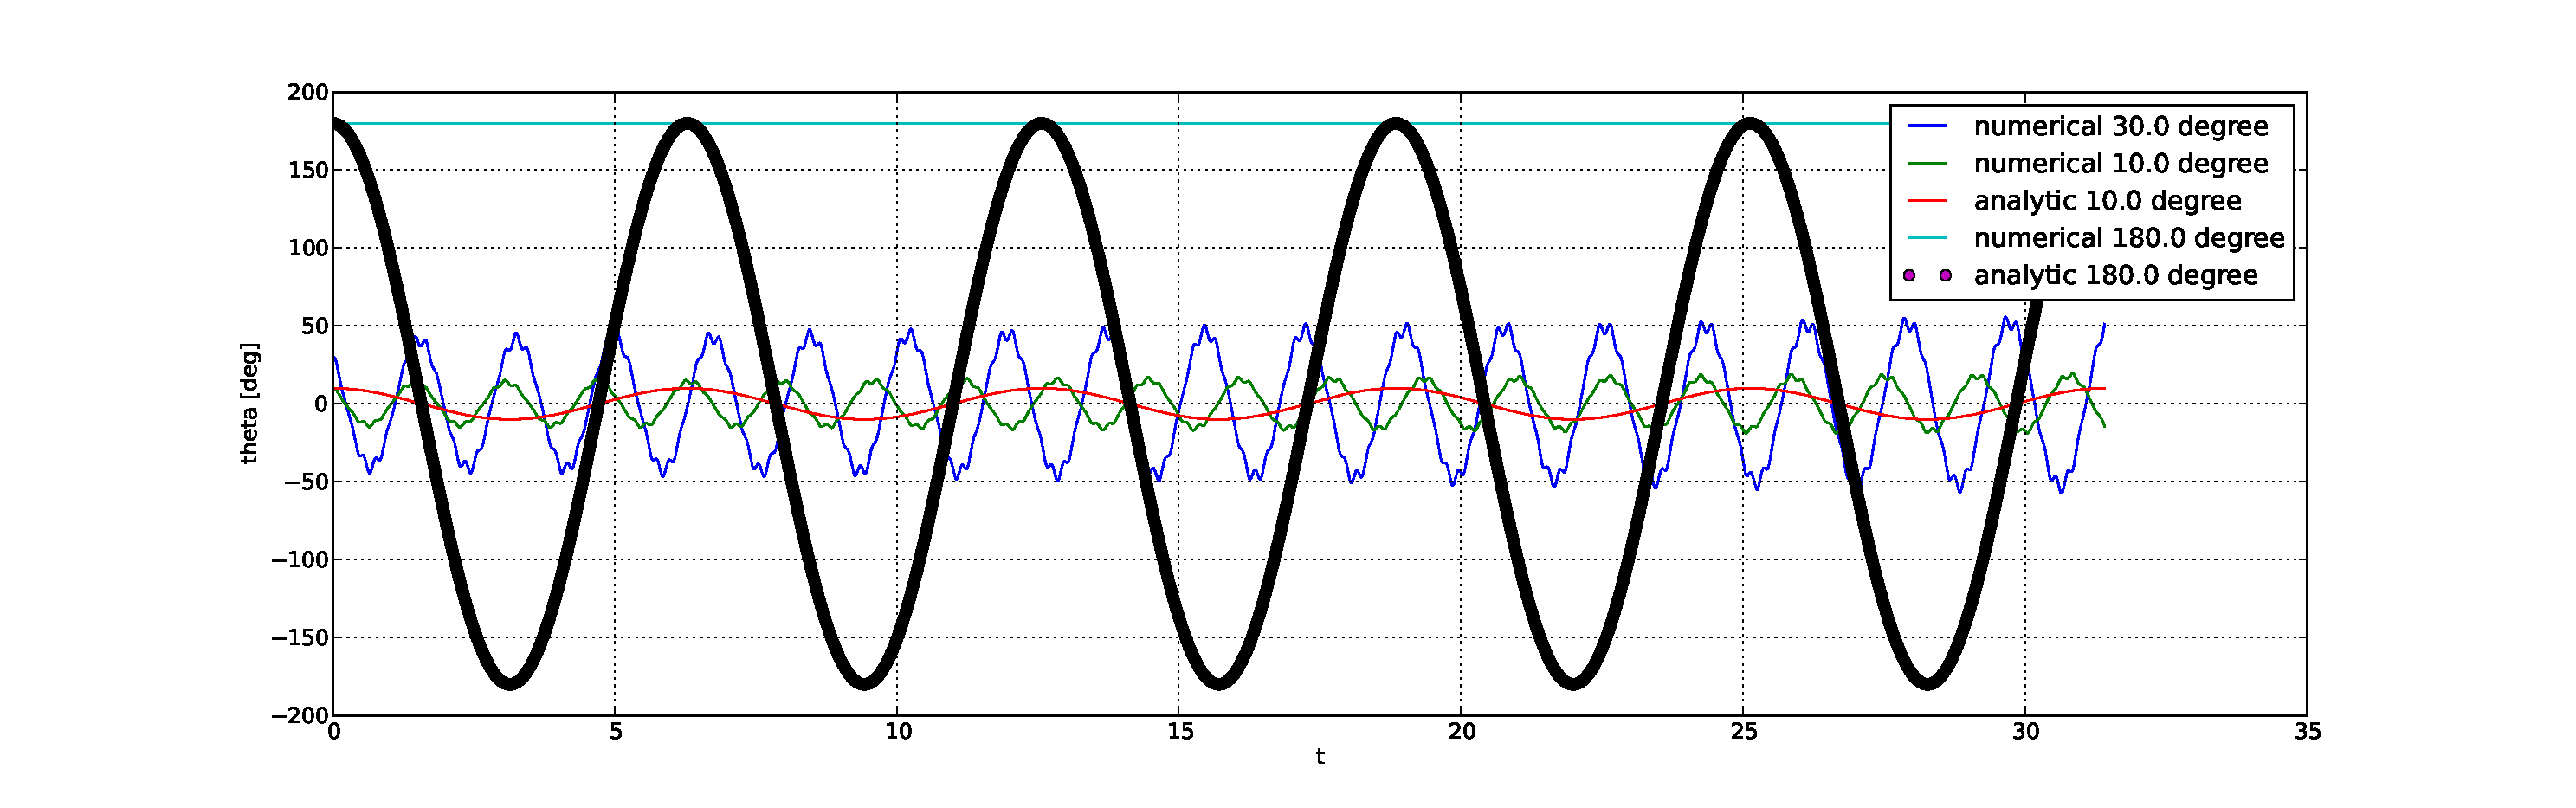
\includegraphics[max size={\textwidth}{\textheight}]{hw5b.eps}
\caption{Plots of the pendulum with different values of $\theta$, with $T$ = $0.2$, $A_o$ = 100, and $L$ = 1}
}
\end{figure}
\noindent As you can see, the pendulum start to be stable when $\theta$ = 180 degree and starts to ossillate around that.\\

\begin{figure}[H]
\centering{
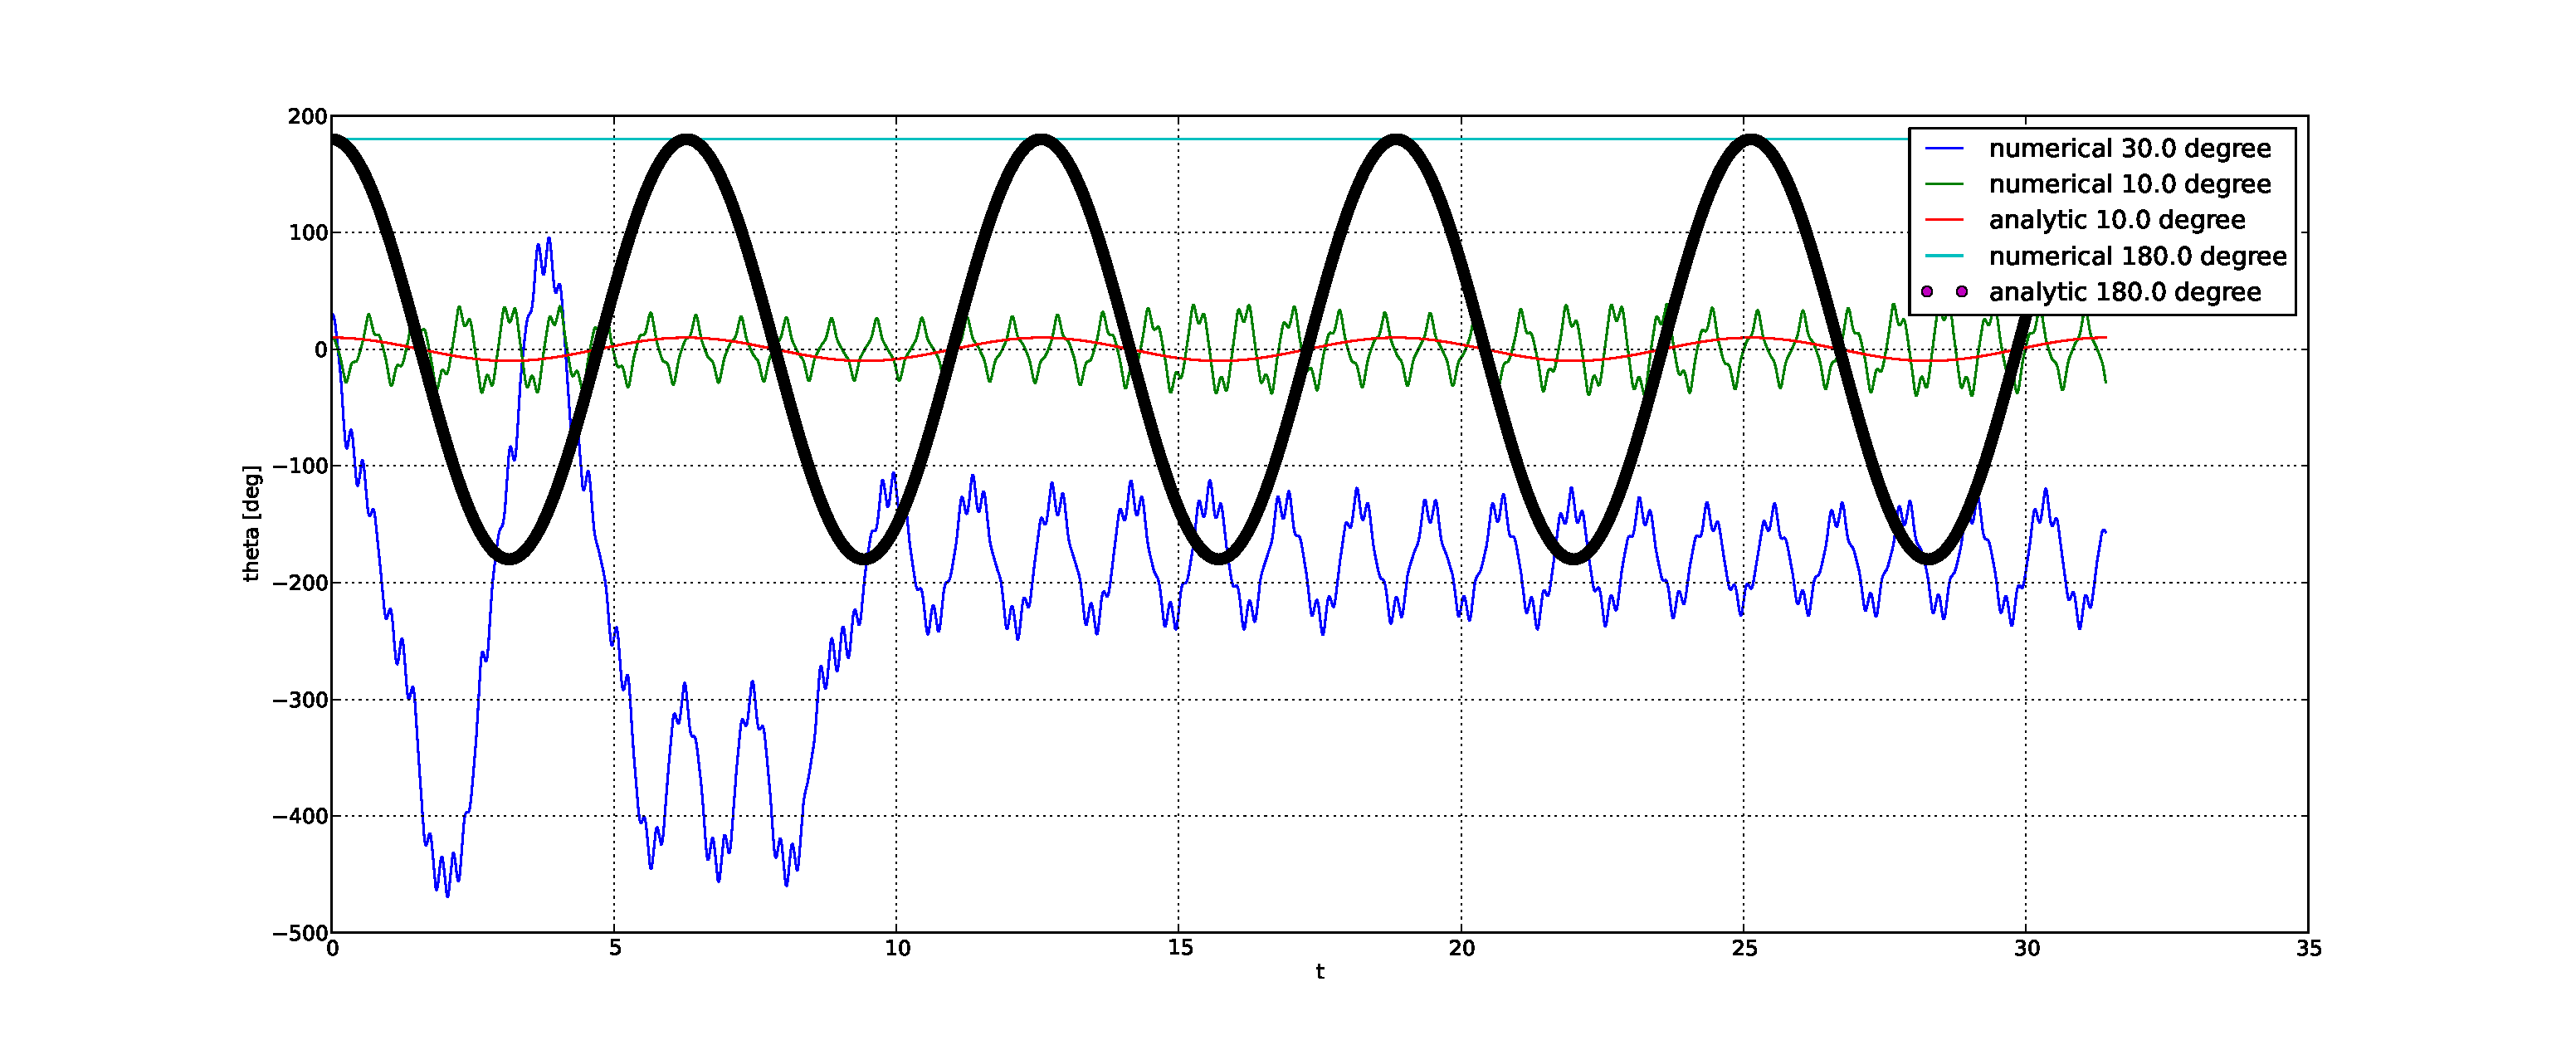
\includegraphics[max size={\textwidth}{\textheight}]{hw5c.eps}
\caption{Plots of the pendulum with different values of $\theta$, with $T$ = $0.2$, $A_o$ = 300, and $L$ = 1}
}
\end{figure}
\noindent This is the plot with $A_o$ = 300, which is $>>$ g.

\end{document}